% =========================================================
% Chapter 7 — Experimental Results
% =========================================================

All experiments were performed with the sensor connected to PMOD~JA on the Nexys Video board, the XADC VAUX0 differential input carrying the sensor analog output, and the Python host application communicating over UART at 115200~baud. Unless stated otherwise, the default timing parameters were used: \texttt{exposure\_us}~=~100~$\mu$s, \texttt{dwell\_us}~=~100~$\mu$s, \texttt{reset\_us}~=~10~$\mu$s, \texttt{cds\_delay\_us}~=~2~$\mu$s.

\section{Timing Verification}

The control signals generated by the sensor FSM were verified by probing the PMOD~JA header with an oscilloscope. The signals \texttt{nRES}, \texttt{nTX}, \texttt{AX[2:0]}, and \texttt{AY[2:0]} were captured during a full-frame scan at default timing parameters.

Figure~\ref{fig:ctrl_signals} shows \texttt{nRES} and \texttt{nTX} during the RESET and INTEGRATE phases. The \texttt{nRES} pulse width and the \texttt{nTX} assertion duration were measured and compared against the configured register values. 
Table~\ref{tab:timing_measured} summarises the comparison.

% ---- FIGURE: nRES and nTX control signals ----
% Use: figures/scope/ctrl_signal_test_1_scope/print_00.png
%      figures/scope/ctrl_signal_test_1_scope/print_01.png
\begin{figure}[h]
  \centering
  % 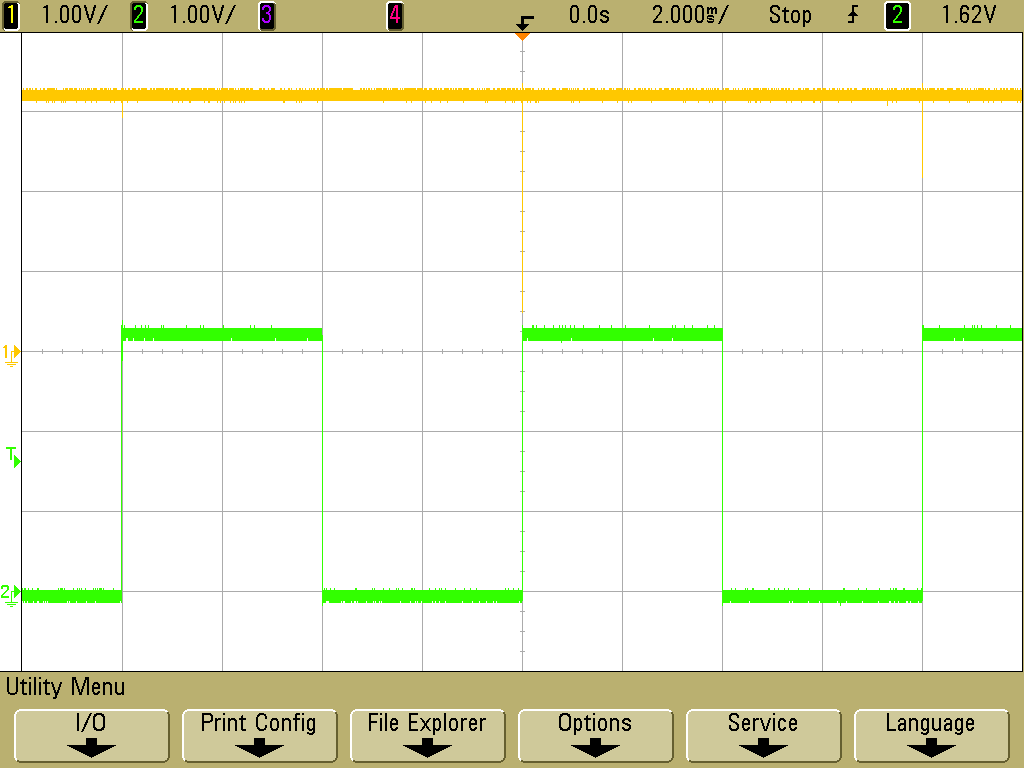
\includegraphics[width=0.8\textwidth]{figures/scope/ctrl_signal_test_1_scope/print_00.png}
  \caption{Oscilloscope capture of \texttt{nRES} and \texttt{nTX}
    during a single scan cycle. \texttt{nRES} is asserted low during
    the RESET phase; \texttt{nTX} is asserted low during INTEGRATE.}
  \label{fig:ctrl_signals}
\end{figure}

\begin{table}[h]
\centering
\caption{Configured vs.\ measured control signal timing.}
\label{tab:timing_measured}
\begin{tabular}{lrr}
\hline
\textbf{Parameter} & \textbf{Configured} & \textbf{Measured} \\
\hline
Reset hold (\texttt{reset\_us}) & 10~$\mu$s  & \\ % TODO: measure \\
Exposure time (\texttt{exposure\_us}) & 100~$\mu$s & \\ % TODO: measure \\
Pixel dwell (\texttt{dwell\_us}) & 100~$\mu$s & \\ % TODO: measure \\
\hline
\end{tabular}
\end{table}